Tous les codes de cette leçon sont comme pour la dernière leçon dans le projet "numalgoplotter" qui est basé sur les codes fournis sur moodle. 

\subsection{Question 1}
\lstinputlisting{numalgoplotter/CubicSplinePlotter.java}

\begin{figure}[H]
	\centering
	\caption{\label{comparaison} Comparaison entre NewtonPlotter (en bleu) et CubicSplinePlotter (en noir)}
	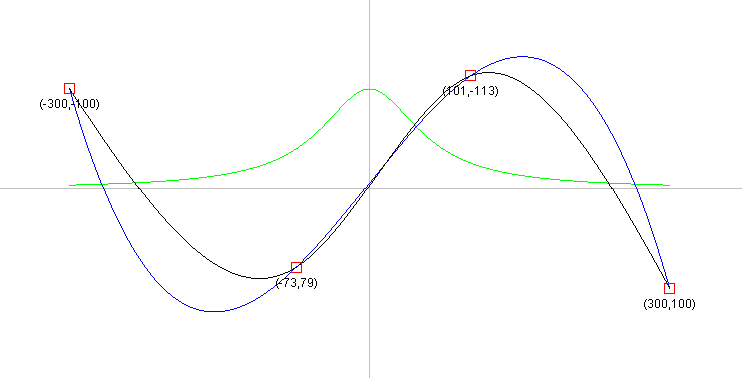
\includegraphics[scale = 0.4]{7_comparaisonNewtonCubic.png}
\end{figure}

\subsection{Question 2}

// TO DO


\subsection{Question 3}

// TO DO


\subsection{Question 4}

// TO DO